\documentclass[a4paper,10pt,twoside]{article}
\usepackage[utf8]{inputenc}
\usepackage[french]{babel}
\usepackage[T1]{fontenc}
\usepackage{amsmath}
\usepackage{amsfonts}
\usepackage{amssymb}
\usepackage{graphicx}
\usepackage{multicol}
\usepackage{array}
\usepackage{float}
\usepackage{epstopdf}
\usepackage[justification=centering]{caption}
\usepackage{caption}
\usepackage{subfig}
\usepackage{gensymb}
\usepackage[bottom]{footmisc}
\usepackage{appendix}
\usepackage{pdfpages}
\usepackage{todonotes}
\usepackage{mathpazo}
\usepackage{titleps}
\usepackage{color}
\usepackage{hyperref}
\usepackage[skins]{tcolorbox}
\usepackage{sectsty}
\usepackage[arrowmos]{circuitikz}
\usepackage{pgfplots}
\usepackage{blindtext}
\usepackage{adjustbox}
\usepackage{listings}
\usepackage[inner=2.5cm,outer=2.5cm,top=3cm,bottom=3cm]{geometry}

\graphicspath{{pictures/}}
\setlength\parindent{0pt}
\renewcommand*\rmdefault{ppl}
\newcolumntype{C}[1]{>{\centering\let\newline\\\arraybackslash\hspace{0pt}}m{#1}}
\newcolumntype{R}[1]{>{\raggedright\arraybackslash}p{#1}}
\sectionfont{\large}
\subsectionfont{\normalsize}

% Page style definitions
\newpagestyle{main}{
	\sethead[Club ELEC : Hands-on 2][][]  % even
			{\chaptertitle}{}{Club ELEC : Hands-on 2}
	\headrule
    \setfoot[\thepage][][]
    		{}{}{\thepage}
}

\newpagestyle{appendix}{
	\sethead[Club ELEC : Annexes][][]  % even
			{}{}{Club ELEC : Annexes}
	\headrule
    \setfoot[\thepage][][]
    		{}{}{\thepage}
    \footrule
}

%----------------------------------------------------------------------------------------
%	TITLE SECTION
%----------------------------------------------------------------------------------------
\title{
	\vspace{2.5cm}
	\normalfont \normalsize
	\huge Club ELEC\\
	\vspace{2.5cm}
	\huge Projet Robot\\
	\vspace{.25cm}
	\Large HO2 - Télécommande infrarouges et programmation
	\vspace{2.5cm}
	\centering
}

\begin{document}
\renewcommand{\figurename}{Fig.}
\renewcommand{\thepage}{\roman{page}}
\setcounter{page}{1}

\pagenumbering{gobble}
\maketitle
\newpage
\pagenumbering{arabic}
\pagestyle{main}

\newpage
\null
\thispagestyle{empty}
\newpage
\clearpage

\setcounter{page}{1}

%%% Introduction
\section*{Introduction}
\section{Introduction}

Grâce au HO2, vous avez été réussi à transformer un signal sonore en un signal carré en utilisant principalement un compareteur, un diviseur résistif et un NE555. L'allure de ces signaux est présentée à la Figure~\ref{fig:signal-all}. En principe, votre circuit fonctionne donc comme attendu, bien joué !

\begin{figure}[h!]
    \centering
    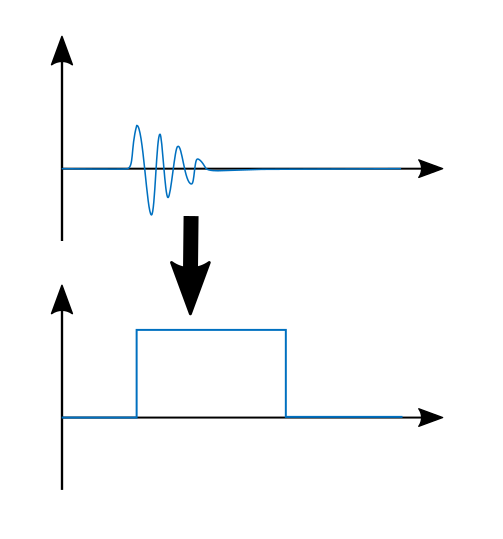
\includegraphics[width=0.5\textwidth]{signals.PNG}
    \caption{Transformation du signal HO2}
    \label{fig:signal-all}
\end{figure}

Maintenant, il va falloir utiliser ce signal carré pour générer le signal de commande: celui-ci doit passer de 0[V] à 5[V] ou de 5[V] à 0[V] lorsqu'un signal carré est généré par un évènement sonore. Vous devez donc reproduire le signal de la Figure~\ref{fig:signal-all_HO3}. Cela vous permettra \textit{in fine} d'utiliser un interrupteur (transitor) connecté à une LED afin de l'allumer ou l'éteindre. Le signal orange à la Figure~\ref{fig:signal-all_HO3} est donc bel et bien votre \textbf{signal de commande}. \\

\begin{figure}[h!]
    \centering
    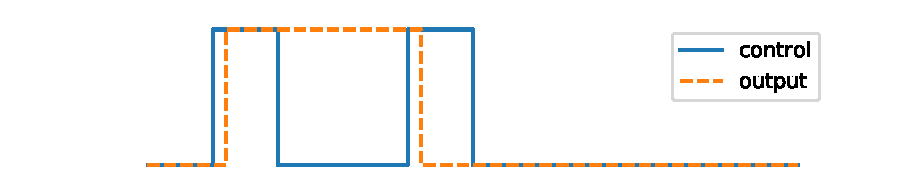
\includegraphics[width=1\textwidth]{figures/signals_control.pdf}
    \caption{Transformation du signal HO3}
    \label{fig:signal-all_HO3}
\end{figure}

%%% Objectifs du HO1
\section*{Objectifs}
% Objectifs: prise en main du micro et du signal sonore, notion AC/DC, utilisation de l'oscilloscope, découplage AC

Les objectifs du premier hands-on sont:

\begin{itemize}
	\item[-] De se familiariser avec le matérial de base (breadboard, multimètre, oscilloscope) et les composants de base (résistances, capacités, amplificateurs opérationnels, composants intégrés) propres à l'électronique.
	\item[-] De comprendre le fonctionnement du micro qui assure la transduction du signal sonore en signal électrique.
	\item[-] De faire le lien entre le signal obtenu et son contenu fréquentiel afin de comprendre la notion de filtrage.
	\item[-] De comprendre la notion AC/DC et le découplage AC.
	\item[-] D'implémenter en pratique la première partie du circuit (micro, filtre et découplage).
\end{itemize}

\begin{figure}[!ht]
	\centering
	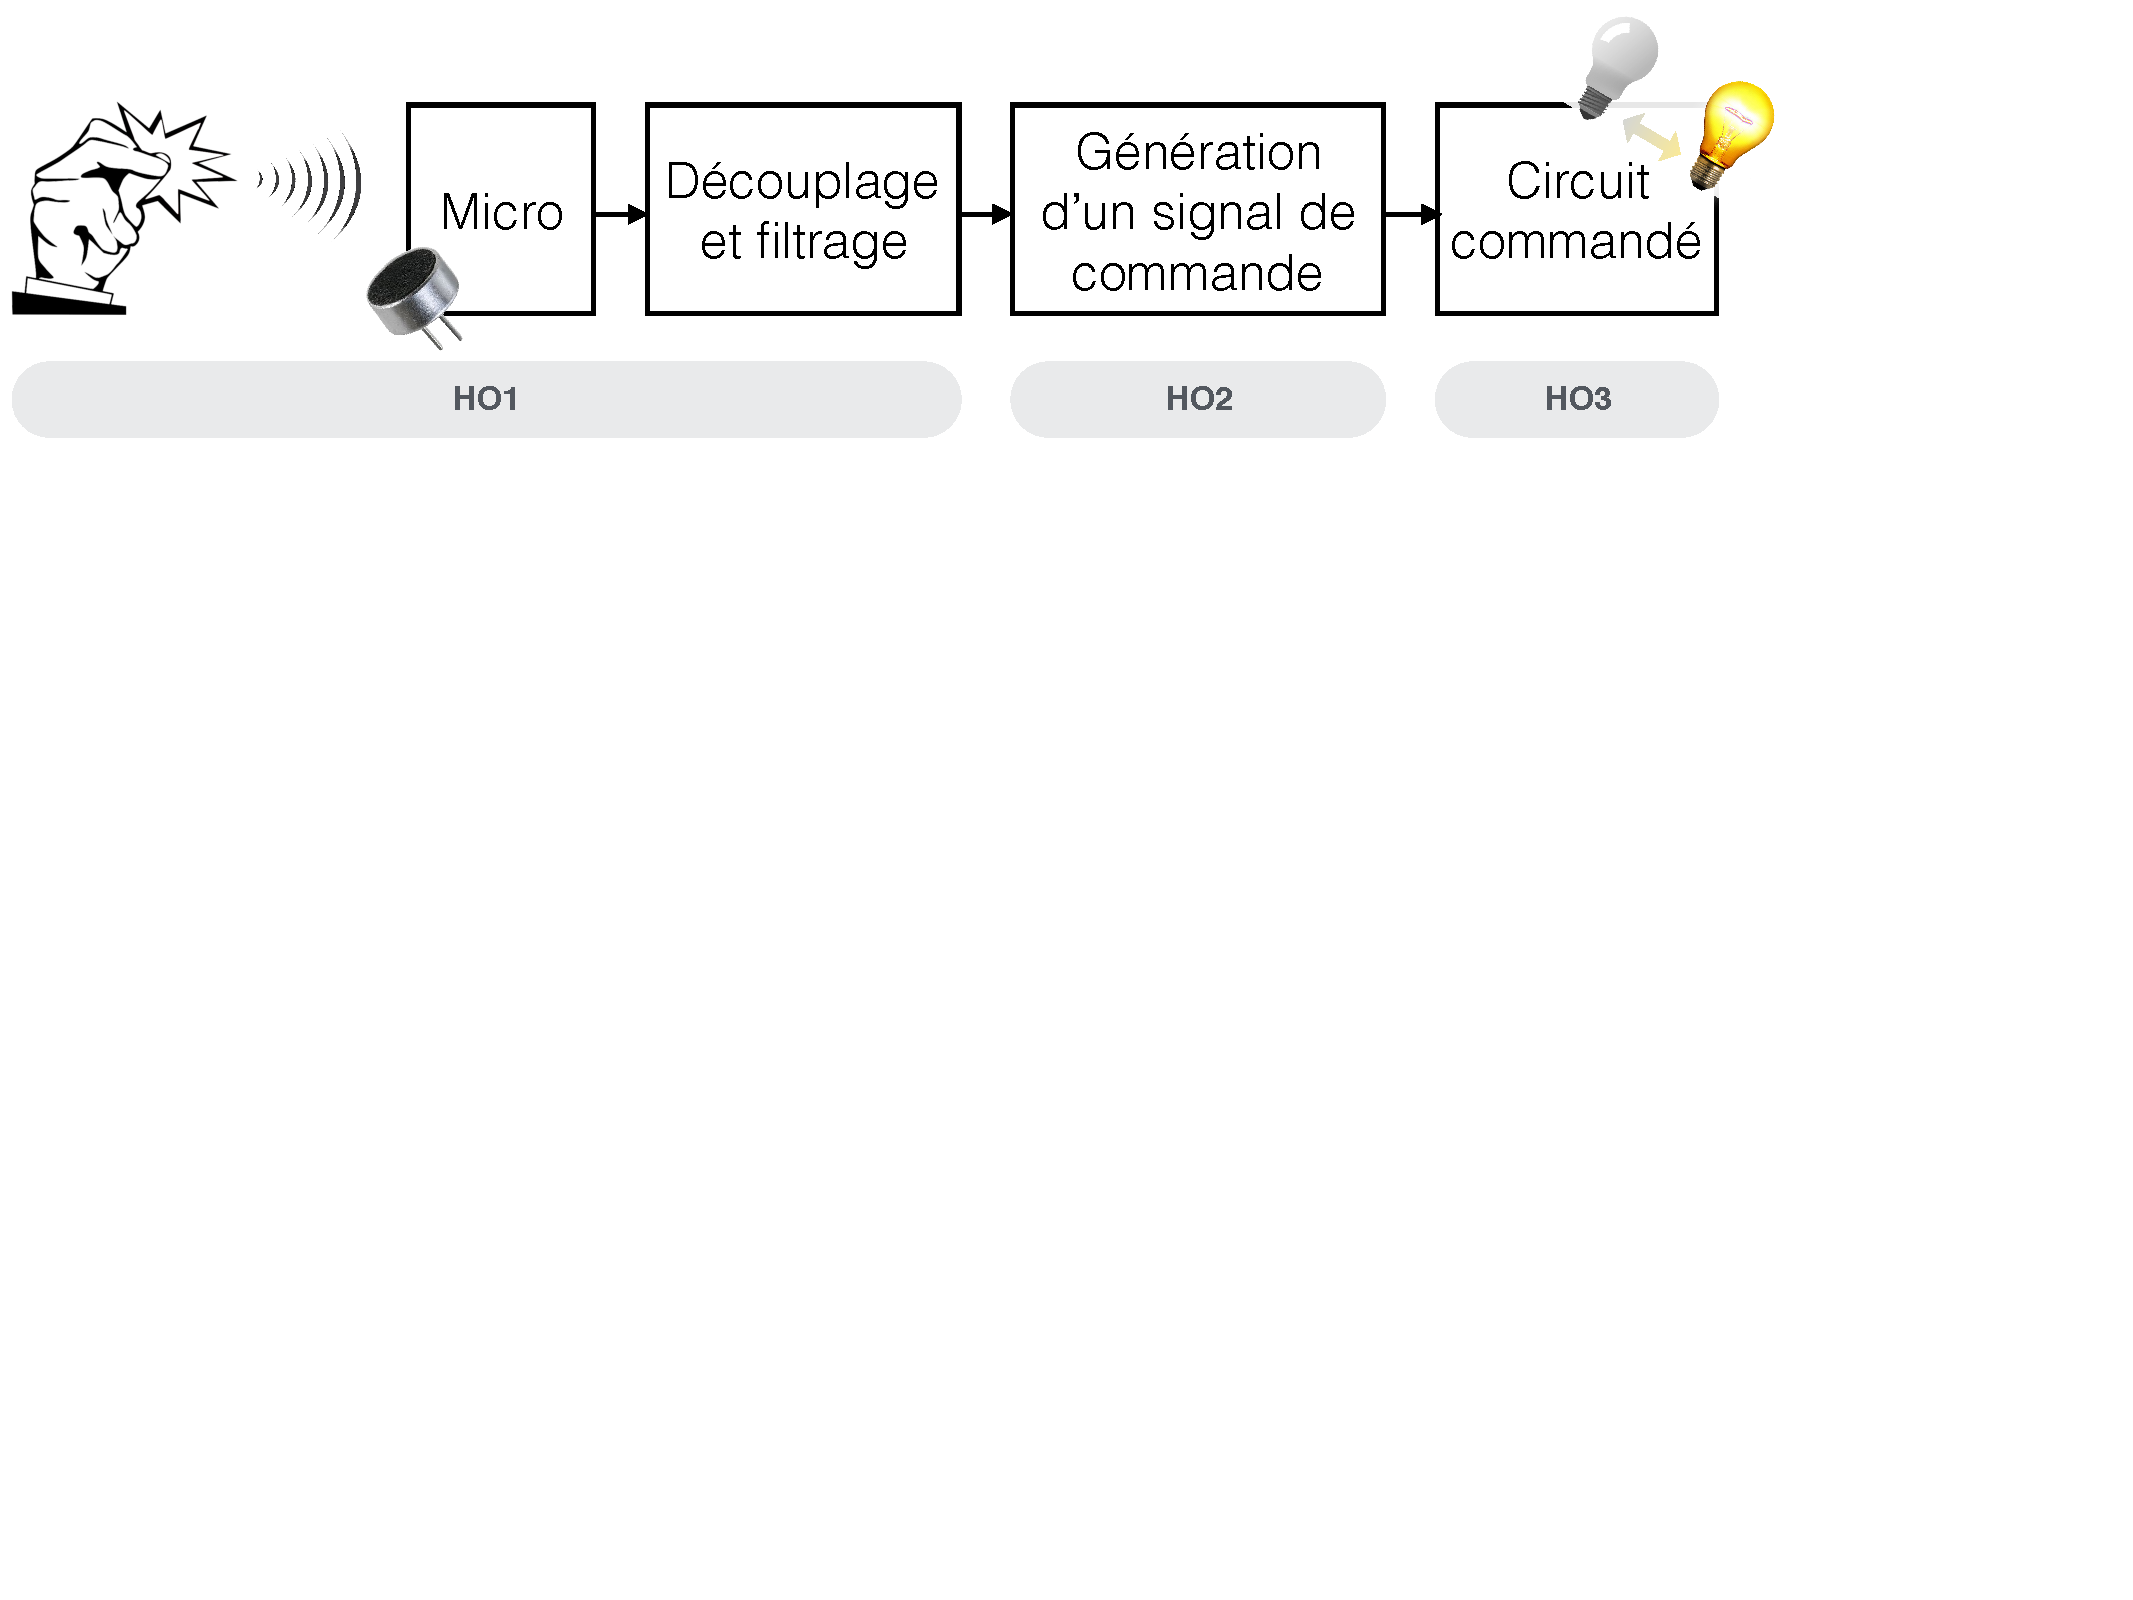
\includegraphics[width=.75\textwidth]{figures/SchemaBloc.pdf}
	\caption{Schéma-bloc du circuit.}
	\label{fig:block-diagram}
\end{figure}

Le schéma-bloc du circuit est présenté à la Figure \ref{fig:block-diagram}. Les ondes acoustiques générées par le claquement de doigt sont captées par le micro qui les transforme en un signal électrique (transduction). Ce signal est ensuite découplé et filtré à l'aide d'un filtre RC, comme présenté plus loin dans ce document. La génération d'un signal de commande propre ainsi que l'implémentation d'un circuit commandé seront abordées plus en détail dans les prochain hands-on.


%%% Description du circuit
\section*{Installations nécessaires}
%%% Installations
Afin de pouvoir programmer votre module Arduino Nano, plusieurs étapes sont nécessaires.

Il vous faut d'abord \textbf{télécharger et installer le programmateur Arduino}. Celui-ci est aussi appelé Arduino IDE (Arduino Integrated Development Environment). Voici les instructions à suivre :
\begin{enumerate}
	\item se rendre sur la page principale du site Arduino (\url{www.arduino.cc/}) ;
	\item cliquer sur l'onglet "Software > Downloads" ; 
	\item choisir votre version d'Arduino IDE (voir Fig. \ref{fig:arduino_ide}) et la télécharger ;
	\item une fois le téléchargement effectué, il ne vous reste plus qu'à installer le programmateur.
\end{enumerate}

\begin{figure}[ht!]
	\centering
	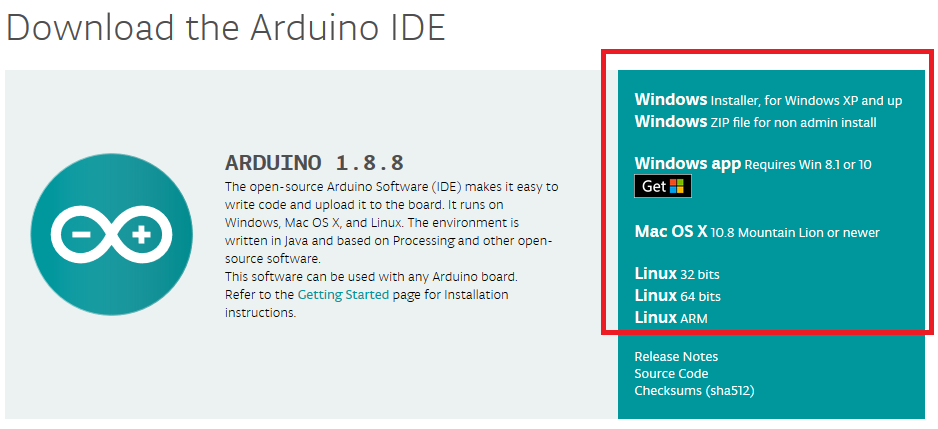
\includegraphics[width=\textwidth]{imgs/arduino_ide.png}
	\caption{Téléchargement du programmateur Arduino.}
	\label{fig:arduino_ide}
\end{figure}

Pour la suite de la séance, il vous faudra également \textbf{installer la librairie IRremote}. Cette librairie gère l'interfaçage avec le récepteur infrarouges et permettra à votre Arduino Nano de correctement recevoir les données envoyées par la télécommande infrarouges. Voici les instructions à suivre :
\begin{enumerate}
	\item ouvrir l'Arduino IDE fraichement installé ;
	\item aller dans \textit{Sketch --> Include Library --> Manage Libraries...} ;
	\item taper "IRremote" dans la barre de recherche ;
	\item cliquer sur la librairie "IRremote" (voir Fig. \ref{fig:arduino_IRremote}) et l'installer ;
	\item voilà ! 
\end{enumerate}

\begin{figure}[ht!]
	\centering
	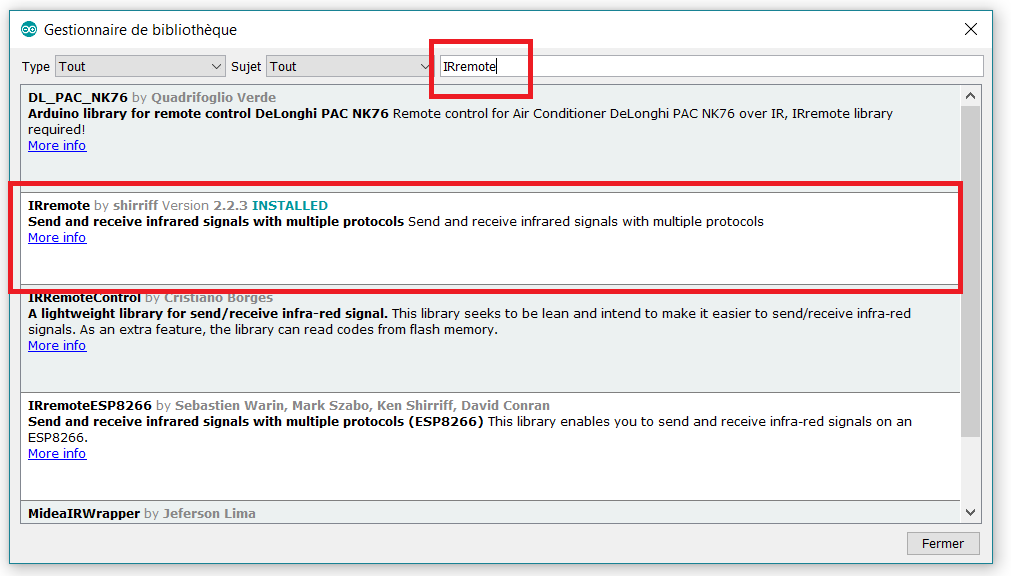
\includegraphics[width=\textwidth]{imgs/arduino_IRremote.png}
	\caption{Installation de la librairie IRremote.}
	\label{fig:arduino_IRremote}
\end{figure}

Enfin, avant de programmer votre module Arduino, il faut s'assurer que certaines configurations soient bien faites dans l'IDE Arduino: d'abord le type de module Arduino que nous allons programmer (Nano dans notre cas), ensuite le type de processeur existant sur ce module (ATmega328P dans notre cas). Voici comment faire pour choisir ces paramètres:
\begin{enumerate}
	\item aller dans \textit{Tools --> Board} et choisir \textit{Arduino Nano} comme type de module Arduino à utiliser (voir Figure \ref{fig:arduino_board}).
	\item aller dans \textit{Tools --> Processor} et choisir \textit{ATmega328P} comme processeur (voir Figure \ref{fig:arduino_processor}).
\end{enumerate}

\begin{figure}[ht!]
	\centering
	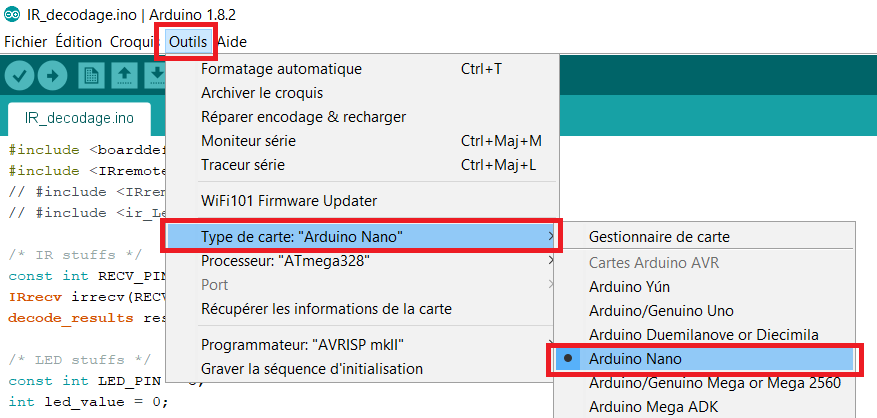
\includegraphics[width=\textwidth]{imgs/arduino_board_v2.png}
	\caption{Choix du type de module Arduino.}
	\label{fig:arduino_board}
\end{figure}

\begin{figure}[ht!]
	\centering
	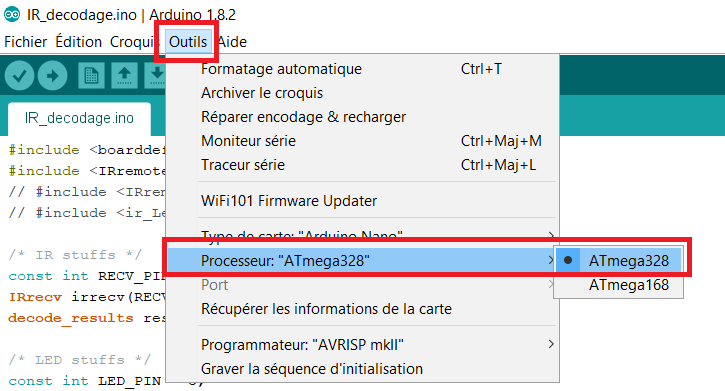
\includegraphics[width=\textwidth]{imgs/arduino_processor_v2.png}
	\caption{Choix du type de processeur sur le module Arduino.}
	\label{fig:arduino_processor}
\end{figure}

Vous êtes enfin prêts à programmer votre module Arduino. Vous l'aurez remarqué, Arduino est open-source et gratuit. Sachez aussi qu'il existe une floppée de librairies existantes pour faire à peu près n'importe quoi !









%Les moteurs utilisés pour ce projet sont des moteurs DC à balais. Ce type de moteur ne nécessite qu'une source de tension DC pour l'alimenter, au contraire de moteurs synchrones ou asynchrones, basés sur des alimentations triphasées ou N-phasées.\\
%
%\begin{minipage}[t]{.45\textwidth}
%	\centering
%	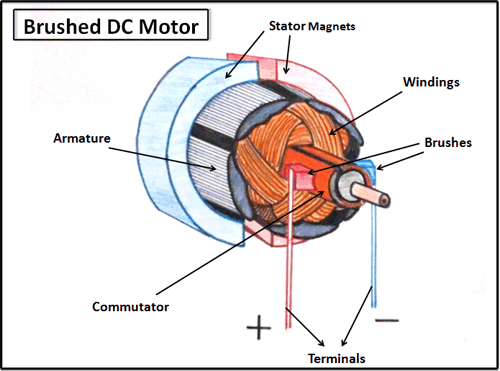
\includegraphics[width=\textwidth]{dc_motor}
%	\captionof{figure}{Schéma d'un moteur DC.}
%	\label{fig:dc_motor}
%\end{minipage}
%\hfill
%\begin{minipage}[t]{.45\textwidth}
%	\centering
%	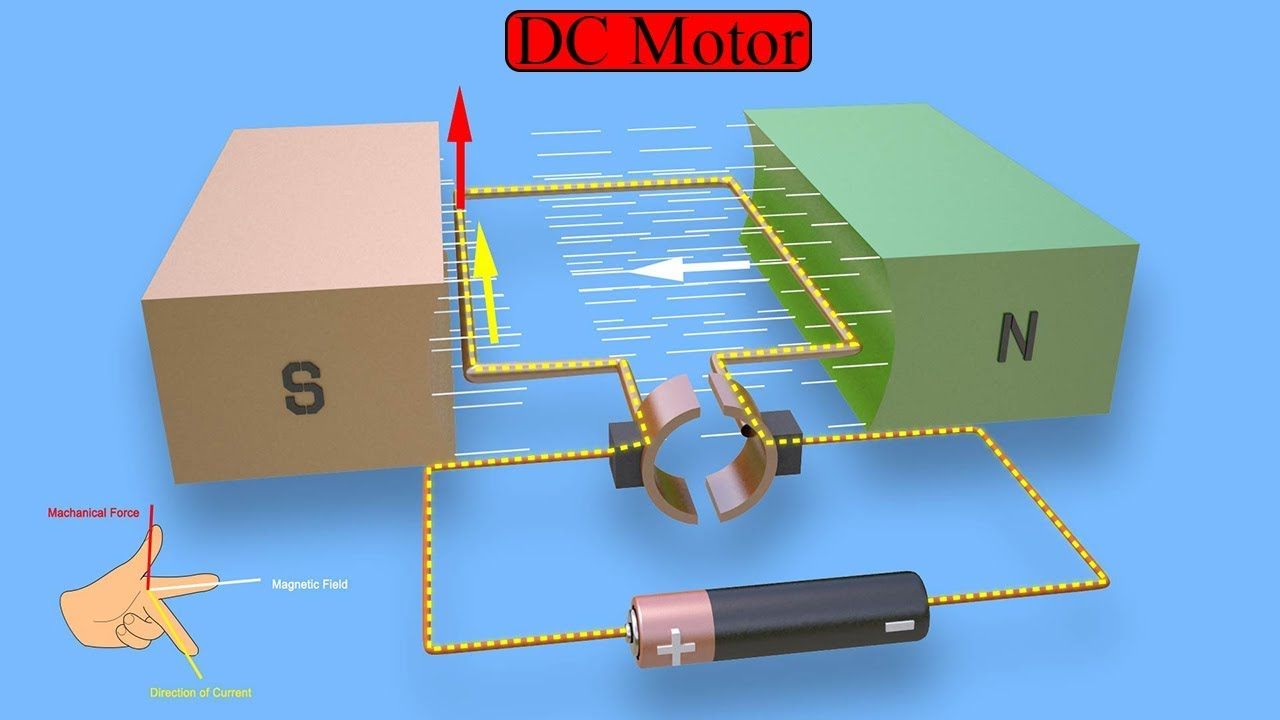
\includegraphics[width=\textwidth]{dc_motor_principle}
%	\captionof{figure}{Principle de fonctionnement du moteur DC.}
%	\label{fig:dc_motor_principle}
%\end{minipage}
%\vspace{.25cm}
%
%Le moteur est constitué de deux pièces principales, comme illustré à la Figure \ref{fig:dc_motor}. D'une part, un \textbf{stator}, élément fixe du moteur, sur lequel on trouve généralement une structure formée d'aimants permanents, servant à générer un champ magnétique de direction fixe. D'autre part, un \textbf{rotor}, élément mobile du moteur, sur lequel on trouve généralement des bobinages alimentés par la tension DC fournie au moteur, servant à générer un champ magnétique de direction variable.\\
%
%Le couple électro-mécanique produit par le moteur résulte du moment de force qui tend à aligner les directions des champs magnétiques générés respectivement par les aimants permanents au stator et les bobinages au rotor, comme représenté à la Figure \ref{fig:dc_motor_principle}. Un commutateur auquel les bobinages sont connectés au travers d'un système de balais, permet de choisir quels bobinages alimenter, de façon à constamment désaligner le champ magnétique résultant des bobinages par rapport à celui des aimants. C'est ce principe qui permet de produire un mouvement rotatif continu.\\
%
%D'un point de vue purement électrique (et pour votre information uniquement, pas besoin de comprendre les détails), le fonctionnement du moteur DC est régi par 2 équations principales:
%
%\begin{align*}
%	\left \lbrace
%	\begin{aligned}
%		V_a &= R_a I_a + L_a \frac{dI_a}{dt} + k \phi \omega_m\\
%		C_{em} &= I \frac{d\omega_m}{dt} = k \phi I_a
%	\end{aligned}
%	\right. 
%\end{align*}
%
%La \textbf{première équation} relie la tension d'alimentation du moteur, notée $V_a$, au courant circulant dans les bobinages, noté $I_a$ et à la force électromotric induite (le terme $k \phi \omega_m$) qui fait directement intervenir la vitesse de rotation du moteur $\omega_m$. La \textbf{seconde équation} relie le couple électro-mécanique, noté $C_{em}$ et proportionel à la dérivée de la vitesse de rotation $\frac{d\omega_m}{dt}$, au courant dans les bobinages.\\
%
%La conclusion principale à tirer de ces équations est qu'il est possible de contrôler la vitesse du moteur $\omega_m$ uniquement en modulant la tension $V_a$ appliquée au moteur.

\clearpage
\newpage
%%% Montage du circuit
\section*{Interfaçage de composants autour de l'Arduino Nano}
Le circuit que nous allons utiliser aujourd'hui se compose de quatre éléments:
\begin{enumerate}
  \item D'une télécommande infrarouges
  \item Récepteur infrarouges
  \item Une led
  \item L'Arduino qui est le \textit{"cerveau"} du système. Il allume la Led quand la télécommande lui demande.
\end{enumerate}

Pour que tout ceci fonctionne, la première étape est d'assembler tout ces composants sur une breadboard. Le schéma du circuit est disponible à la \ref{fig:circuit}.

\begin{figure}[!t]
\centering
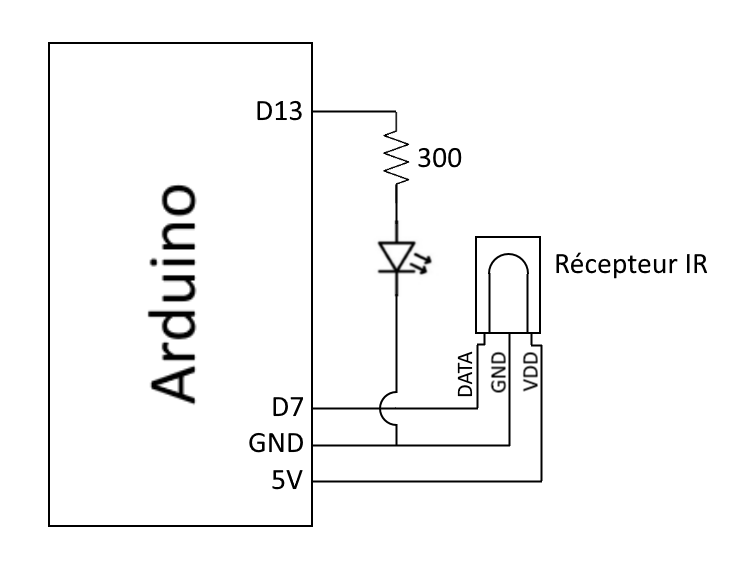
\includegraphics[width=0.8\textwidth]{imgs/circuit.png}
\caption{Circuit à réaliser pour contrôler l'Arduino grâce à une télécommande infrarouge.}
\label{fig:circuit}
\end{figure}


%%% Programme pour récupérer les codes envoyés par la télécommande
\section*{Premier programme: récupération des codes envoyés par la télécommande}
Le but de cet exercice est d'établir une communication entre votre télécommande et l'Arduino. Typiquement, quand votre télécommande essaye de communiquer avec votre télévision, cela se passe 3 étapes:
\begin{enumerate}
  \item Quand vous appuyez sur un bouton, la télécommande envoie une valeur $X$
  via infrarouges.
  \item La télévision reçoit cette valeur $X$ via le récepteur infrarouges.
  \item En fonction de la valeur de $X$, le microcontrôleur de la télévision fait une action. Il peut
  soit augmenter le volume, changer de chaîne ou encore s'éteindre.
\end{enumerate}

La toute première étape est donc de savoir quelle valeur est envoyée par votre télécommande quand vous appuyez sur un certain bouton. Le programme \autoref{code1} permet de faire cela. En quelques mots, à chaque fois que l'Arduino reçoit un message infrarouges, il l'envoie directement à l'ordinateur. Cela vous permet donc de savoir le code correspondant à chacun des boutons de votre télécommande (notez ça sur un feuille ;)).

Pour voir les messages en console, vous devez aller dans \textit{Tools-->Serial Monitor}.

\lstset{language=C}
\begin{lstlisting}[frame=single,numbers=left,numberstyle=\small,label={code1},caption={Lecture de la télécommande}]
#include <IRremote.h>

const int RECV_PIN = 7;

IRrecv irrecv(RECV_PIN);
decode_results results;

void setup(){
  Serial.begin(9600);
  irrecv.enableIRIn();
}

void loop(){
  if (irrecv.decode(&results)){
        Serial.println(results.value, HEX);
        irrecv.resume();
  }
}
\end{lstlisting}


%%% Programme pour allumer/éteindre une LED lorsqu'on appuie sur une touche de la télécommande
\section*{Second programme: contrôle d'une LED avec la télécommande}
Une fois que vous avez identifié le code que votre télécommande envoie pour un certain bouton, vous pouvez adapter l’exemple \autoref{code2}.
Ici, à chaque itération de la fonction \textit{loop()}, l'Arduino regarde si le récepteur infrarouges a reçu une message. Pour chaque message reçu, il regarde à quel bouton ce code correspond (ici $AB456CD$ pour le bouton 1 et $05FBAC33$ pour le bouton 2). Ensuite, il exécute une fonction correspondant au bouton utilisé (\textit{IR\_button1()}).
Dans le cas du bouton 1, la Led s'allume ou s'éteint à chaque fois que le bouton est appuyé.

\lstset{language=C}
\begin{lstlisting}[frame=single,numbers=left,numberstyle=\small,label={code2},caption={Code 2}]
  #include <IRremote.h>

  #define REMOTE_BUTTON1    0xAB456CD   // Ligne a modifier
  #define REMOTE_BUTTON2    0x5FBAC33   // Ligne a modifier

  const int RECV_PIN = 7;
  const int LED_PIN = 13;

  IRrecv irrecv(RECV_PIN);
  decode_results results;

  int LED_val = 0;

  void setup() {
    Serial.begin(9600);
    pinMode(LED_PIN,OUTPUT);
    digitalWrite(LED_PIN,LED_val);
    irrecv.enableIRIn();
    delay(500);
  }

  void loop() {
    if (irrecv.decode(&results)){
      //Serial.println(results.value, HEX);
      irrecv.resume();
      switch (results.value) {
        case REMOTE_BUTTON1:
          IR_button1();
          break;
        case REMOTE_BUTTON2:
          IR_button2();
          break;
      }
      irrecv.resume();
      }
  }

  void IR_button1(){
      LED_val = 1-LED_val;
      digitalWrite(LED_PIN,LED_val);
  }

  void IR_button2(){
    // faire qqch
  }
\end{lstlisting}


%%% Contrôle du mouvement d'un robot
\section*{Contrôle du mouvement d'un robot}
Vous avez appris dans ce hands-on à contrôler des moteurs DC à partir de signaux de contrôle digitaux. Dans votre circuit, les valeurs de ces signaux de contrôle étaient fixées manuellement. Pour la suite de ce projet, vous recevrez, entre autres, un microcontrôleur de type Arduino qui permet d'envoyer des signaux de contrôle 5V, ainsi que 2 moteurs DC, un L293D et une pile 9V. Imaginez dès à présent la stratégie la plus efficace pour contrôler les mouvements de votre robot à partir de ce matériel. Voici quelques questions pour vous aiguiller:
\begin{itemize}
\item Quels sont les signaux à envoyer au L293D pour avancer? Et pour reculer?
\item Comment contrôler chacun des moteurs pour tourner?
\item Comment faire pour régler la vitesse du robot? 
\end{itemize}

%%%% Installations
%\section{Installations nécessaires}
%Avant de pouvoir programmer votre balise réceptrice, plusieurs étapes sont nécessaires.
%
%Il vous faut d'abord \textbf{télécharger et installer le programmateur Arduino}. Celui-ci est aussi appelé Arduino IDE (Arduino Integrated Development Environment). Voici les instructions à suivre :
%\begin{enumerate}
%	\item se rendre sur la page principale du site Arduino (\url{www.arduino.cc/}) ;
%	\item cliquer sur l'onglet "Software" ;
%	\item choisir votre version d'Arduino IDE (voir Fig. \ref{fig:arduino_ide}) et la télécharger ;
%	\item une fois le téléchargement effectué, il ne vous reste plus qu'à installer le programmateur.
%\end{enumerate}
%
%\begin{figure}[ht!]
%	\centering
%	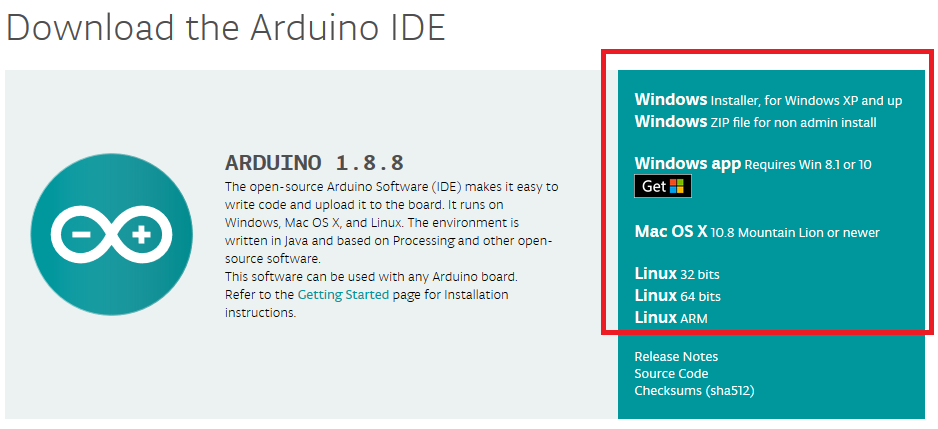
\includegraphics[width=\textwidth]{imgs/arduino_ide.png}
%	\caption{Téléchargement du programmateur Arduino.}
%	\label{fig:arduino_ide}
%\end{figure}
%
%Patience, avant de programmer il vous reste encore quelques étapes. En effet, une fois l'IDE installé, il vous faudra également \textbf{installer la librairie RF24}. Celle-ci permettra à votre module Arduino Nano de communiquer correctement avec le module RF qui y est connecté . Voici les instructions à suivre :
%\begin{enumerate}
%	\item ouvrir l'Arduino IDE fraichement installé ;
%	\item aller dans \textit{Sketch --> Include Library --> Manage Libraries...} ;
%	\item taper "RF24" dans la barre de recherche ;
%	\item cliquer sur la librairie "RF24" (voir Fig. \ref{fig:arduino_RF24}) et l'installer ;
%	\item voilà !
%\end{enumerate}
%
%\begin{figure}[ht!]
%	\centering
%	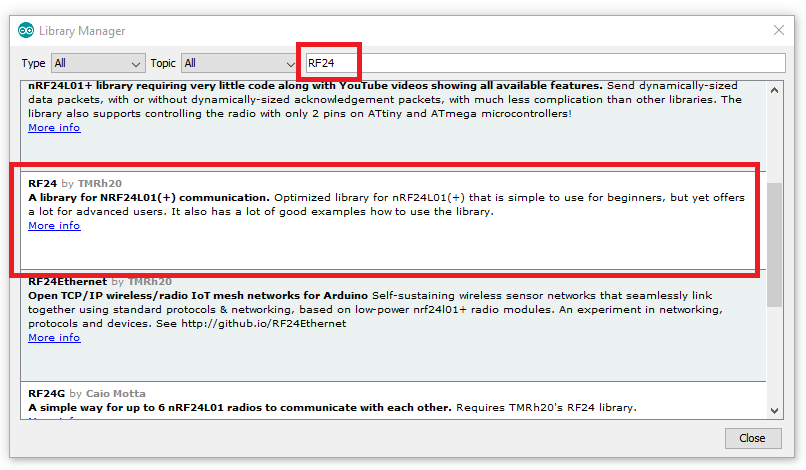
\includegraphics[width=\textwidth]{imgs/arduino_RF24.png}
%	\caption{Installation de la librairie RF24.}
%	\label{fig:arduino_RF24}
%\end{figure}
%
%Vous êtes enfin prêts à programmer votre module Arduino. Vous l'aurez remarqué, Arduino est open-source et gratuit. Sachez aussi qu'il existe une floppée de librairies existantes pour faire à peu près n'importe quoi !
%
%%%% Principe de fonctionnement
%\section{Votre premier programme Arduino !}
%Pour vous aider à vous lancer dans le fabuleux monde de la programmation Arduino, voici quelques instructions pour lancer le code exemple pour votre baliser RF réceptrice.
%
%\subsection{Configurations}
%Il y a d'abord quelques étapes préliminaires :
%\begin{enumerate}
%	\item ouvrir l'Arduino IDE ;
%	\item brancher le module Arduino à votre PC via un câble USB ;
%	\item copier le code qui se trouve dans le fichier \textit{reception} fourni dans l'IDE ;
%	\item sauver le croquis (Sketch en anglais) en allant dans \textit{File --> Save} ou simplement en appuyant sur \textit{CTRL + S} ;
%\end{enumerate}
%
%Le résultat devrait être proche de celui de la Fig. \ref{fig:arduino_reception}.
%
%\begin{figure}[ht!]
%	\centering
%	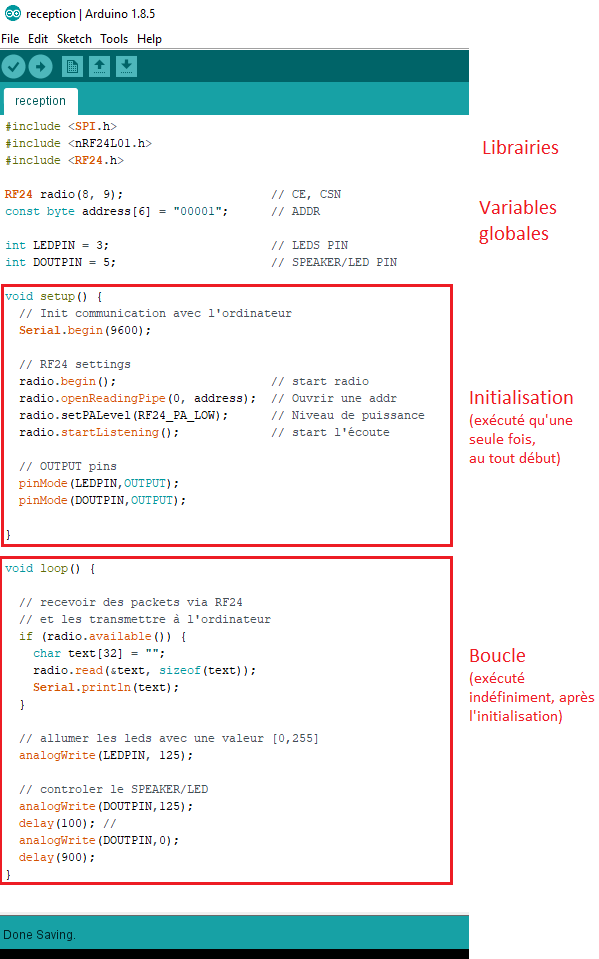
\includegraphics[width=0.6\textwidth]{imgs/arduino_reception.png}
%	\caption{Exemple de code récepteur que nous vous fournissons.}
%	\label{fig:arduino_reception}
%\end{figure}
%
%Avant de programmer le module, il y a encore quelques configurations à effectuer :
%\begin{enumerate}
%	\setcounter{enumi}{3}
%	\item choisir la bonne "board", pour qu'elle corresponde à "Arduino Nano" ; pour cela, aller dans \textit{Tools --> Board --> Arduino Nano} (voir Fig. \ref{fig:arduino_board}) ;
%	\item choisir le bon processeur, pour qu'il corresponde à "ATmega328P" ; pour cela, aller dans \textit{Tools --> Processor --> ATmega328P} (voir Fig. \ref{fig:arduino_processor}) ;
%	\item choisir le bon port série ; pour cela, aller dans \textit{Tools --> Port} et choisir le port série adéquat (il n'y en a qu'un si vous n'avez qu'une seule connection USB) ;
%	\item voilà, il est temps de programmer votre module Arduino ; il suffit de cliquer sur \textit{Sketch --> Upload} ou d'utiliser \textit{CTRL + U}.
%\end{enumerate}
%
%\begin{figure}[ht!]
%	\centering
%	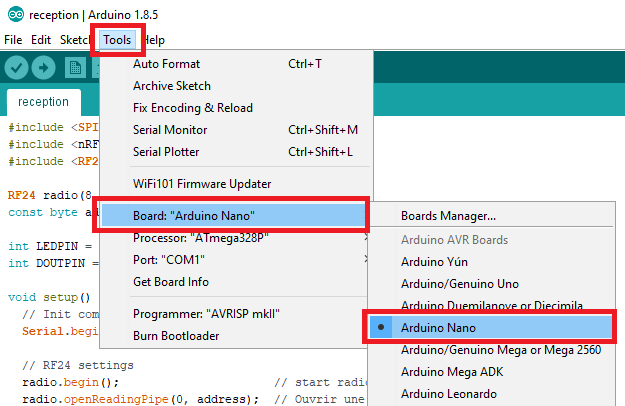
\includegraphics[width=0.6\textwidth]{imgs/arduino_board.png}
%	\caption{Configuration de la "board".}
%	\label{fig:arduino_board}
%\end{figure}
%
%\begin{figure}[ht!]
%	\centering
%	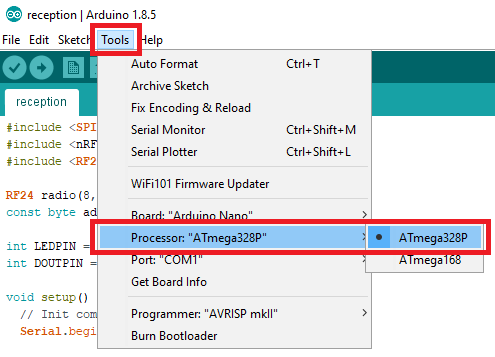
\includegraphics[width=0.6\textwidth]{imgs/arduino_processor.png}
%	\caption{Configuration du processeur.}
%	\label{fig:arduino_processor}
%\end{figure}
%
%Si tout se passe bien, votre carte électronique devrait faire de jolies choses !
%
%\newpage
%\subsection{Explication du code}
%Maintenant que votre carte est programmée, il est important de comprendre ce qu'elle fait. Pour cela, il suffit de comprendre le code repris à la Fig. \ref{fig:arduino_reception}. Le code est structuré en plusieurs parties, comme repris sur la figure :
%\begin{enumerate}
%	\item d'abord, on inclut les \textbf{librairies} utiles ; dans notre cas, la librairie "RF24", qui a besoin également de deux autres librairies ;
%	\item ensuite, on définit plusieurs \textbf{variables globales} ; par exemple, \texttt{LEDPIN = 3} indique que la pin 3 de l'Arduino est utilisée pour allumer les LEDs, via le LED driver ;
%	\item la fonction \texttt{setup} sert d'\textbf{initialisation} et n'est exécutée qu'une seule fois, au tout début (quand on branche l'alimentation par exemple) ; dans cette fonction :
%		\begin{itemize}
%			\item le moniteur série est configuré (ce dernier permet d'envoyer du texte à l'ordinateur ; pour l'activer, il suffit d'aller dans \textit{Tools --> Serial Monitor}) ;
%			\item la radio est configurée (canal, adresse, etc.) ;
%			\item les pins de sortie de l'Arduino sont configurées (LEDs et buzzer) ;
%		\end{itemize}
%	\item enfin, la fonction \texttt{loop} est la \textbf{partie centrale du code} ; cette fonction est exécutée indéfiniment après la phase d'initialisation ; dans le code d'exemple :
%		\begin{itemize}
%			\item on attend de recevoir un message et on le transmet vers l'ordinateur via le port série ;
%			\item on allume les LEDs via le LED driver ;
%			\item on allume la LED seule ou le buzzer pendant un petit moment.
%			\item et on recommence la fonction \texttt{loop} !
%		\end{itemize}
%\end{enumerate}
%
%\section{Conclusion}
%À partir de maintenant, vous pouvez partir du code exemple et le modifier à votre guise. Votre tâche est de recevoir correctement les messages émis par la balise émetrice pour pouvoir la localiser correctement.
%
%Voici quelques derniers conseils pour mener à bien votre mission:
%\begin{itemize}
%	\item nous vous avons fourni le code de l'émetteur (fichier \textit{transmit}) ; nous vous conseillons de bien le comprendre pour mettre en place votre stratégie de localisation !
%	\item quand vous utilisez les pins de l'Arduino, pour par exemple allumer une LED, vérifiez toujours que cette LED est bien connectée à la pin que vous choisissez dans le code.
%	\item posez des questions, n'hésitez surtout pas, nous sommes là pour cela !
%\end{itemize}
%
%\begin{center}
%Que la force soit avec vous !
%\end{center}

\end{document}
